A typical problem where this tool can help the programmer is solving (partial) differential equations in two dimensions with iterative methods. We will look at a very simplified model of the distribution of heat, e.g. in a metal plate.
As we cannot simulate the distribution for every point on the plate, we discretize the problem, obtaining a grid which can be represented by a matrix. The boundary values are invariant throughout the entire simulation process. We assume that the heat value for an inner node is the mean of the four adjoining nodes (which are either inner nodes or nodes on the boundary). The inner values are iteratively computed using a red-black scheme as marked in the following picture (we assume a $5 \times 5$ matrix):

\begin{figure}[h]
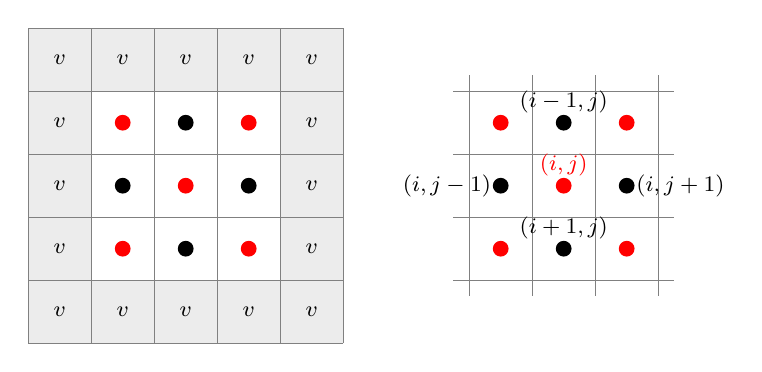
\begin{tikzpicture} [scale=0.8,font=\footnotesize]
	\fill [gray!15] (-2,-2) rectangle +(1,5);
	\fill [gray!15] (2,-2) rectangle +(1,5);
	\fill [gray!15] (-2,-2) rectangle +(5,1);
	\fill [gray!15] (-2,2) rectangle +(5,1);
	\draw [step=1cm,gray] (-2,-2) grid ++(5,5);
	
	\fill [color=red] (.5,.5) circle [radius=.125cm];
	\fill [color=red] (-.5,-.5) circle [radius=.125cm];
	\fill [color=red] (-.5,1.5) circle [radius=.125cm];
	\fill [color=red] (1.5,1.5) circle [radius=.125cm];
	\fill [color=red] (1.5,-.5) circle [radius=.125cm];
	\fill [color=black] (-.5,.5) circle [radius=.125cm];
	\fill [color=black] (.5,1.5) circle [radius=.125cm];
	\fill [color=black] (.5,-.5) circle [radius=.125cm];
	\fill [color=black] (1.5,.5) circle [radius=.125cm];
	
	\node at (-1.5,2.5) {$v$};
	\node at (-.5,2.5) {$v$};
	\node at (.5,2.5) {$v$};
	\node at (1.5,2.5) {$v$};
	\node at (2.5,2.5) {$v$};
	\node at (2.5,1.5) {$v$};
	\node at (2.5,.5) {$v$};
	\node at (2.5,-.5) {$v$};
	\node at (2.5,-1.5) {$v$};
	\node at (1.5,-1.5) {$v$};
	\node at (.5,-1.5) {$v$};
	\node at (-.5,-1.5) {$v$};
	\node at (-1.5,-1.5) {$v$};
	\node at (-1.5,-.5) {$v$};
	\node at (-1.5,.5) {$v$};
	\node at (-1.5,1.5) {$v$};
	
	% 
	\node (offset) at (6,0) {};
	\draw [step=1cm,gray] (-1.25+6,-1.25) grid ++(3.5,3.5);
	
	\fill [red] (.5,.5) +(offset) circle [radius=.125cm] node [above] {$(i,j)$};
	\fill [red] (-.5,-.5) +(offset) circle [radius=.125cm];
	\fill [red] (-.5,1.5) +(offset) circle [radius=.125cm];
	\fill [red] (1.5,1.5) +(offset) circle [radius=.125cm];
	\fill [red] (1.5,-.5) +(offset) circle [radius=.125cm];
	\fill [black] (-.5,.5) +(offset) circle [radius=.125cm] node [left] {$(i,j-1)$};
	\fill [black] (.5,1.5) +(offset) circle [radius=.125cm] node [above] {$(i-1,j)$};
	\fill [black] (.5,-.5) +(offset) circle [radius=.125cm] node [above] {$(i+1,j)$};
	\fill [black] (1.5,.5) +(offset) circle [radius=.125cm] node [right] {$(i,j+1)$};
\end{tikzpicture}
\end{figure}

One iteration consists of an update of all black nodes and an update of all red nodes. Thus we can implement the updates in one iteration as follows:
\begin{lstlisting}
// update inner black nodes
for(i=1; i<N-1; i++)
   for(j=1+(i%2); j<N-1; j+=2)
      m[i][j] = ( m[i-1][j] + m[i+1][j] 
                + m[i][j-1] + m[i][j+1] )/4.0;

// update inner red nodes
for(i=1; i<N-1; i++)
  for(j=1+((i+1)%2); j<N-1; j+=2)
      m[i][j] = ( m[i-1][j] + m[i+1][j] 
                + m[i][j-1] + m[i][j+1] )/4.0;
\end{lstlisting}
In the above implementation, all the red or black nodes in one row are updated before we jump to the next row. Alternatively, we could update the nodes by columns. Whether updates by columns instead of updates by rows make any difference can be decided with the help of the tool. Furthermore, it can visualize the access patterns; in this example, one obvious pattern consists of the four accesses to the adjoining matrix entries (in a fixed order).

Another very similar example is the following Jacobi method, where we use two grids/matrices $A$ and $B$ instead of the red-black update order (only parts of the two grids are depicted):
\begin{figure}[h]
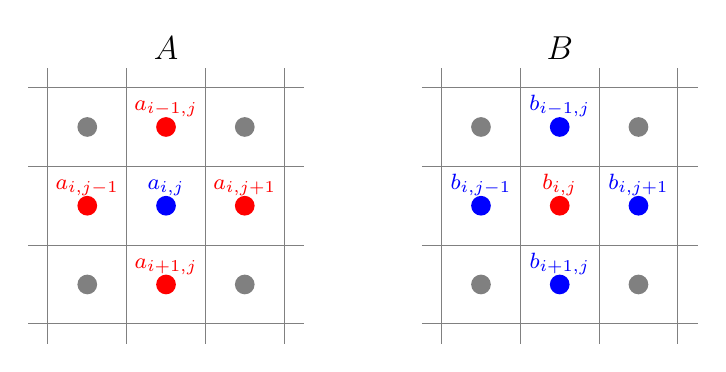
\begin{tikzpicture} [font=\footnotesize]
	\draw [step=1cm,gray] (-1.25,-1.25) grid ++(3.5,3.5);
	
	\fill [blue] (.5,.5) circle [radius=.125cm] node [above] {$a_{i,j}$};
	\fill [gray] (-.5,-.5) circle [radius=.125cm];
	\fill [gray] (-.5,1.5) circle [radius=.125cm];
	\fill [gray] (1.5,1.5) circle [radius=.125cm];
	\fill [gray] (1.5,-.5) circle [radius=.125cm];
	\fill [red] (-.5,.5) circle [radius=.125cm] node [above] {$a_{i,j-1}$};
	\fill [red] (.5,1.5) circle [radius=.125cm] node [above] {$a_{i-1,j}$};
	\fill [red] (.5,-.5) circle [radius=.125cm] node [above] {$a_{i+1,j}$};
	\fill [red] (1.5,.5) circle [radius=.125cm] node [above] {$a_{i,j+1}$};
	
	\node (offset) at (5,0) {};
	\draw [step=1cm,gray] (-1.25+5,-1.25) grid ++(3.5,3.5);
	
	\fill [red] (.5,.5) +(offset) circle [radius=.125cm] node [above] {$b_{i,j}$};
	\fill [gray] (-.5,-.5) +(offset) circle [radius=.125cm];
	\fill [gray] (-.5,1.5) +(offset) circle [radius=.125cm];
	\fill [gray] (1.5,1.5) +(offset) circle [radius=.125cm];
	\fill [gray] (1.5,-.5) +(offset) circle [radius=.125cm];
	\fill [blue] (-.5,.5) +(offset) circle [radius=.125cm] node [above] {$b_{i,j-1}$};
	\fill [blue] (.5,1.5) +(offset) circle [radius=.125cm] node [above] {$b_{i-1,j}$};
	\fill [blue] (.5,-.5) +(offset) circle [radius=.125cm] node [above] {$b_{i+1,j}$};
	\fill [blue] (1.5,.5) +(offset) circle [radius=.125cm] node [above] {$b_{i,j+1}$};
	
	\node [font=\large] at (.5,2.5) {$A$};
	\node [font=\large] at (.5+5,2.5) {$B$};
\end{tikzpicture}
\end{figure}
\\$A$ is the input and output grid, i.e. $A$ is initialized with the initial values and contains the final computed values at the end of the iterations. A naive method could look like this: In one iteration, the entries of $B$ are updated first, using the values in $A$ (marked \textcolor{red}{red}), then $A$ is updated using the (updated) entries from $B$ (marked \textcolor{blue}{blue}):
\begin{lstlisting}
for(i=1; i<N-1; i++)
for(j=1; j<N-1; j++)
   b[i][j] = ( a[i-1][j] + a[i][j-1] 
             + a[i+1][j] + a[i][j+1] )/4.0;

for(i=1; i<N-1; i++)
for(j=1; j<N-1; j++)
   a[i][j] = ( b[i-1][j] + b[i][j-1] 
             + b[i+1][j] + b[i][j+1] )/4.0;
\end{lstlisting}
However, the tool will reveal that other update methods are more efficient in terms of cache usage: For example, we could first update the minimal number of rows in $B$ until we can update the next row in $A$ which has not been updated yet in the current iteration. Then we move on to the next not-yet-updated row in $B$ etc. The advantage of such an "'interwoven"' update method is that after having updated the rows in $B$, the respective values are still available in the cache memory, so when updating the row in $A$ in the next step, we do not need to load the necessary values of $B$ in the cache again.

We will look at yet another example: We want to compare different implementations of multiplying two square matrices. Let $A$ and $B$ denote the operand matrices and $C$ the product matrix, then we can naively implement the multiplication $C=A \cdot B$ as follows (\texttt{N}-by-\texttt{N} matrices):
\begin{lstlisting}
for(i=0; i<N; i++)
   for(j=0; j<N; j++)
      for(k=0; k<N; k++)
         c[i][j] += a[i][k] * b[k][j];
\end{lstlisting}
The three nested loops can be permutated without changing the result, thus we obtain 6 simple versions of this matrix multiplication algorithm. One could argue that traversing the matrices by rows is more cache-efficient than a traversal by columns as a two-dimensional matrix is stored linearly - row after row - in memory. Thus we can reduce the number of cache loads by ensuring that both $A$ and $B$ are traversed by rows (whereas in the above example $B$ is traversed by columns). The idea is to multiply $A$ not by $B$ but by the transpose of the transpose of $B$, which is mathematically the same:
\begin{lstlisting}
// compute bt = transpose of b
for(i=0; i<N; i++)
   for(j=0; j<N; j++)
      for(k=0; k<N; k++)
         c[i][j] += a[i][k] * bt[j][k];
\end{lstlisting}
Obviously, the index \texttt{k} traverses both operand matrices by rows.

To outline further approaches, there is the possibility to multiply $A$ and $B$ blockwise. Blocking can be done in one or two dimensions, which means that the index range of either one of the inner loops is split into equal intervals (called "'blocks"') or both inner loops are split. (There is no point in using blocking for the outer loop too as the outer index is always the one which changes least.)

